\documentclass[letterpaper,11pt]{report}
\usepackage{float,captdef,multicol}
\usepackage{amssymb,amsmath,amsfonts,fancybox}
%\usepackage[activeacute,spanish,es-tabla]{babel}
\usepackage[spanish]{babel} % English formatting
\usepackage[utf8]{inputenc}
\usepackage[colorlinks]{hyperref}
\usepackage{graphicx}
\usepackage{cancel}
\usepackage{marginnote}
\usepackage{tensor,physics}
\usepackage{xcolor}
\usepackage{biblatex}
\addbibresource{sample.bib}
\hypersetup{colorlinks=true, linkcolor=purple}
%\addbibresource{sample.bib}

\renewcommand*{\marginnotevadjust}{-0.1cm}
\renewcommand*{\marginfont}{\footnotesize}
\usepackage[right=4.5cm,left=2cm,top=3cm,bottom=3.0cm]{geometry}

%\usepackage[notref]{showkeys} % muestra los labels de las referencias.

\spanishdecimal{.}


\begin{document}

\sffamily

\thispagestyle{empty}
\begin{center}

\

\vspace{6.5cm}

\rule{15cm}{0.1cm}

\vspace{1.5cm}

{\huge \textsc{\textbf{Notas sobre Teoría de Cuerdas}}}

\vspace{1.5cm}

\rule{15cm}{0.1cm}

\vspace{1.5cm}

Versi'on del \today

\end{center}


\newpage
\thispagestyle{empty}
\ \\
\newpage
\setcounter{page}{1}
\pagenumbering{roman}

\pagestyle{plain}
\chapter*{Prefacio}
\addcontentsline{toc}{chapter}{Prefacio}
\bigskip
\bigskip
\bigskip
\bigskip
\bigskip
\bigskip
Estas notas han sido escritas por \href{https://github.com/10blackhole/}{ Borja Diez B.} y están lejos de ser un material académico. Las he escrito para estudiar conceptos de física que me parecen interesante. Aún así, comparto el documento para quien le interese. 

La mayor parte de estas notas han sido sacas de \cite{2009fcst.book.....Z}.



\bigskip
\bigskip
\bigskip
\bigskip
\bigskip
\bigskip





\bigskip
\bigskip
\bigskip

\bigskip
\bigskip
\bigskip


\tableofcontents
\pagenumbering{arabic}
\setcounter{page}{1}
\chapter{Una breve introducción}
\section{El camino hacia la unificación}
Cuatro fueras fundamentales han sido reconocidas en la naturaleza. Démosle un vistazo:
\begin{itemize}
    \item \textbf{La fuerza de gravedad}. Esta fuerza fue descubierta por Isaac Newton. La gravedad sufrió una profunda reformulación en la teoría de la Relatividad General de Albert Einstein. En dicha teoría, la arena espacio-temporal de la relatividad especial adquiere vida propia, y las fuerzas gravitacionales emergen de la curvatura de ese espacio-tiempo dinámico. La teoría de Einstein es una teoría clásica de la gravitación. No está formulada como una teoría cuántica.

    \item \textbf{La fuerza electromagnética}. Dicha fuerza es descrita por las ecuaciones de Maxwell. El electromagnetismo, o la teoría de Maxwell, es formulada como una teoría clásica de los campos electromagnéticos. Al contrario que la mecánica Newtoniana, la cuela es modificada por la Relatividad Especial, la teoría de Maxwell es completamente consistente con la Relativiad Especial.

    \item \textbf{La fuerza débil}. Esta fuerza es responsable de los procesos del decaimiento nuclear beta, en el cual un neutrino decae en un protón, un electrón y un antineutrino. En general, procesos que involucran neutrinos están medidos por fueras débiles. Mientras que el decaimiento nuclear beta ha sido conocido desde finales del siglo 19, el reconocimiento de que una nueva fuerza estaba en juego no fue hasta mediados del siglo 20. Las interacciones débiles son muchos más débiles que las interacciones electromagnéticas.

    \item \textbf{La fuerza fuerte}. Hoy en día llamada la fuerza de color. Esta fuerza mantiene juntos los constituyentes de neutrinos, protones, piones, y muchas otras partículas subnucleares. Estos constituyentes, llamados quarks, se mantiene tan apretados por la fuerza de color que ellos no se pueden ver isolados.
\end{itemize}

En los úñtimos 1960s el modelo de Wingberg-Salam para las interacciones \textbf{electrodébiles} juntó el electromagnetismo y la fuerza débil en un marco unificado. Fue necesario para una teoría de las interacciones débiles predictiva y consistente.

La teoría es inicialmente formulada con cuatro partículas sin masa que llevan las fuerzas. Un proceso de quiebre de la simetría les da masa a tres de estas partículas: los $W^+, W^-$ y los $Z^0$ . Estas partículas son las que llevan la fuerza débil. La partícula que queda sin masa es el fotón, que es el que lleva la fuerza electromagnética.

Las ecuaciones de Maxwell son ecuaciones del electromagnetismo clásico. Esta teoría no es ni aproximada ni una teoría correcta para fenómenos microscópicos. La electrodinámica cuántica (QED), la versión cuántica de el electrodinámica clásica, es requerida para calculos correctos en esta arena. En QED el fotón aparece como la cuanto del campo electromagnético. Las teoría de las interacciones débiles es también una teoría cuántica de partículas, entonces lo correcto, la teoría unificada es la teoría electrodébil cuántica.

El proceso de cuantización es también exitoso en el caso de la fuerza de color fuerte, en la teoría resultante es la cromodinámica cuántica (QCD). Los llevadores de la fuerza de color son ocho partículas sin masa. Estas son gluones coloridos, y como los quarks, ellos no pueden ser observados isolados.  Los quarks responden a los gluones porque ellos levan color. Los quarks pueden venir en tres colores.

En resúmen tenemos
\begin{equation}
    \text{Teoría electrodébil} + \text{QCD} = \text{Modelo Estándar de la física de partículas}
\end{equation}

En el Modelos Estándar (SM) hay algunas interacciones entre el sector electrodébil y el QCD porque algunas partículas sienten ambos tipos de fuerzas. El SM resume completamente e conocimiento actual de la física de partículas.

En el Modelo Estándar hay 12 llevadores de fuerza: los 8 gluones, los $W^-,W^+,Z^0$ y el fotón. Todos estos son \textbf{bosones}. También existen varias partículas de materia, todas ellas son \textbf{fermiones}. Las partículas de mateira son de dos tipos: \textbf{leptones}\footnote{Ver \url{https://es.wikipedia.org/wiki/Leptón}} y \textbf{quarks\footnote{Ver \url{https://es.wikipedia.org/wiki/Cuark}}}. Los leptones incluyen el electrón $e^-$, el muon $\mu^-$, el tauón $\tau^-$, y los neutrinos asociados $\nu_e,\nu_\mu$ y $\nu_\tau$. Podemos enlistarlos como
\begin{equation}
    \text{Leptones: } (\nu_e,e^-),\quad (\nu_\mu,\mu^-)\quad\text{y}\quad (\nu_\tau,\tau^-).
\end{equation}
Dado que debemos incluir sus antipartículas, esto suma un total de $12$ leptones. Los quarks llevan la carga de color, carga eléctrica, y responden a la fuerza débil. Hay $6$ tipos diferentres de quarks. Poéticamente llamados sabores, esos tipos son: up($u$), down$(d)$, charm($c$), strange($s$), top($t$) y bottom($b$). Podemos enlistarlos como
\begin{equation}
    \text{Quarks: } (u,d),\quad (c,s),\quad (t,b).
\end{equation}
Cada uno de los $6$ sabores de quarks viene en $3$ colores, así que esto nos da un total de $18$ partículas. Incluyendo sus antipartículas, tenemos un total de $36$ quarks. Sumando los Leptones y Qaurks juntos tenemos un gran total de $48$ partícual de materia.

El Modelos Estándar tiene dos defectos signifcantes:
\begin{itemize}
    \item No incluye la gravedad.
    \item Tiene alrededor de $20$ parámetros que no pueden ser calculados sin su framework. Quizás el ejemplo más simple de tal parámetro es el radio adimensional entre la masa del muón y la del electrón. El valor de este radio es aproximadamente $207$, y tiene que ser puesto en el modelo de forma manual.
\end{itemize}

    Una posibilidad atractiva es que una versión más completa del Modelo Estándar incluya la \textbf{supersimetría}. Esta es una simetría que relaciona bosones(los llevadores de la fuerza) y fermiones(los llevadores de la materia). La supersimetría podría ser una forma de relacionar fuerza y materia.

    \textcolor{purple}{Una \textit{unificación} de la gravedad con las otras fuerzas debe ser requerida para construir una teoría completa!!!}

\subsection{La Teoría de Cuerdas como una teoría unificada de la física}
En la Teoría de Cuerdas,
\begin{enumerate}
    \item Todas las partículas están unificadas
    \item Es una teoría cuántica, y al incluir la gravedad, es una teoría cuántica de la gravedad.
\end{enumerate}

\begin{pregunta}
    ¿Por qué la Teoría de Cuerdas es una teoría unificada?
\end{pregunta}
En la Teoría de Cuerdas, cada partícula está identificada con un modo particular de vibración de una cuerda microscópica elemental.

Uno de los estados de vibración de las cuerdas es el gravitón, el cuanto del campo gravitacional.

\begin{pregunta}
  ¿Estamos seguros de que la Teoría de Cuerdas es una buena teoría cuántica de la gravedad?  
\end{pregunta}
No hay compelta certeza aún, pero la evidencia es muy buena. De hecho, los problemas de incalculabilidad o falta de predictibilidad que ocurren cuando tratamos de cuantizar la teoría de Einstein no aparecen en Teoría de Cuerdas.

La primera señal de que ST es bastante única es que no tiene parámetros adimensionales ajustables. Una teoría que posee tales parámetros no es relamente única. Teoría de Cuerdas tiene un parámetro dimensional, la longitud de la cuerda $l_s$. Su valor puede ser toscamente pensado como el típico tamaño de las cuerdas.

Otra intrigante señal de la unicidad de la Teoría de Cuerdas es el hecho de que la dimensionalidad del espacio-tiempo está fija. Nuestro espacio-tiempo físico es 4-dimensional. En el Modelo Estándar esta información es usada para construir la teoría; no es derivada. Por otro lado, en Teoría de Cuerdas, el número de las dimensiones del espacio-tiempo emerge de un cálculo. La respuesta no es 4, sino que 10. Algunas de esas dimensiones podría estar oculta a simple vista si son enrolladas en un espacio lo suficientemente pequeño para escapar de la detección de experimentos realizados a escalas de bajas energías. Si la Teoría de Cuerdas es correcta, algún mecanismo debe asegurar que la dimensionalidad observable del espacio-tiempo es 4.


\section{Relatividad Especial y dimensiones extra}
Definimos el inérvalo $\Delta s^2$ como
\begin{align}
   \label{2.13} -\Delta s^2&\equiv -(\Delta x^0)^2+(\Delta x^1)^2+(\Delta x^2)^2+(\Delta x^3)^2\\
    \Delta s^2&=\Delta s'^2
\end{align}

Una notación útil puede ser motivada al tratar de simplificar la expresión para el intervalo invariante $\dd s^2$. Para hacer esto, introducimos símbolos que llevan subíndices en vez de superíndices. Definamos
\begin{equation}
    \dd x_0\equiv -\dd x^0,\qquad \dd x_{i}\equiv\dd x^{i},\quad i=1,2,3
\end{equation}
El único cambio significantes es la inclusión del signo menos para la componente cero. Escribiendo todo junto,
\begin{equation}
    \dd x_\mu=(\dd x_0,\dd x_1,\dd x_2,\dd x_3)\equiv(-\dd x^0,\dd x^1,\dd x^2,\dd x^3)
\end{equation}
Ahora podemos reescribir $\dd s^2$ en términos de $\dd x^\mu$ y $\dd x_\mu$:
\begin{align}
    -\dd s^2&=-(\dd x^0)^2+(\dd x^1)^2+(\dd x^2)^2+(\dd x^3)^2\\
    &=\dd x_0\dd x^0+\dd x_1\dd x^1+\dd x_2\dd x^2+\dd x_3\dd x^3
\end{align}
y vemos que el signo menos en (\ref{2.13}) se va. El intervalo invariante entonces queda
\begin{equation}
    -\dd s^2=\sum_{\mu_0}^3\dd x_\mu \dd x^\mu=\dd x_\mu\dd x^\mu
\end{equation}
donde hemos usado la convención de suma de Einstein, la cual nos que índices repetidos a diferentes alturas se suman.

Podemos también expresar $\dd s^2$ usando la métrica de Minkowski $\eta_{\mu\nu}$,
\begin{equation}
    \eta_{\mu\nu}=\eta_{\nu\mu}=\mqty(\dmat[0]{-1,1,1,1})=\eta^{\mu\nu}
\end{equation}

Cualquier objeto con dos índices $M_{\mu\nu}$ puede ser descompuesto en una parte simétrica y una parte antisimétrica:
\begin{equation}
    M_{\mu\nu}=\frac{1}{2}(M_{\mu\nu}+M_{\nu\mu})+\frac{1}{2}(M_{\mu\nu}-M_{\nu\mu})
\end{equation}

La métrica de Minkowski puede ser usada para \textit{bajar índices}:
\begin{equation}
    \dd x_\mu=\eta_{\mu\nu}\dd x^\nu
\end{equation}
Otras propiedad a notar son
\begin{align}
    a^\mu b_\mu&=a_\mu b^\mu\\
    \eta^{\nu\rho}\eta_{\rho\mu}&=\delta^\nu_\mu
\end{align}

Las transformaciones de Lorentz son las relaciones entre coordenadas en dos sistemas de referencia inerciales diferentes. Consideremos un marco de referencia $S$ y otro $S'$, que se está moviendo a lo largo del eje $x$ positivo del marco $S$ con velocidad $v$.
\begin{figure}[h!]
    \centering
    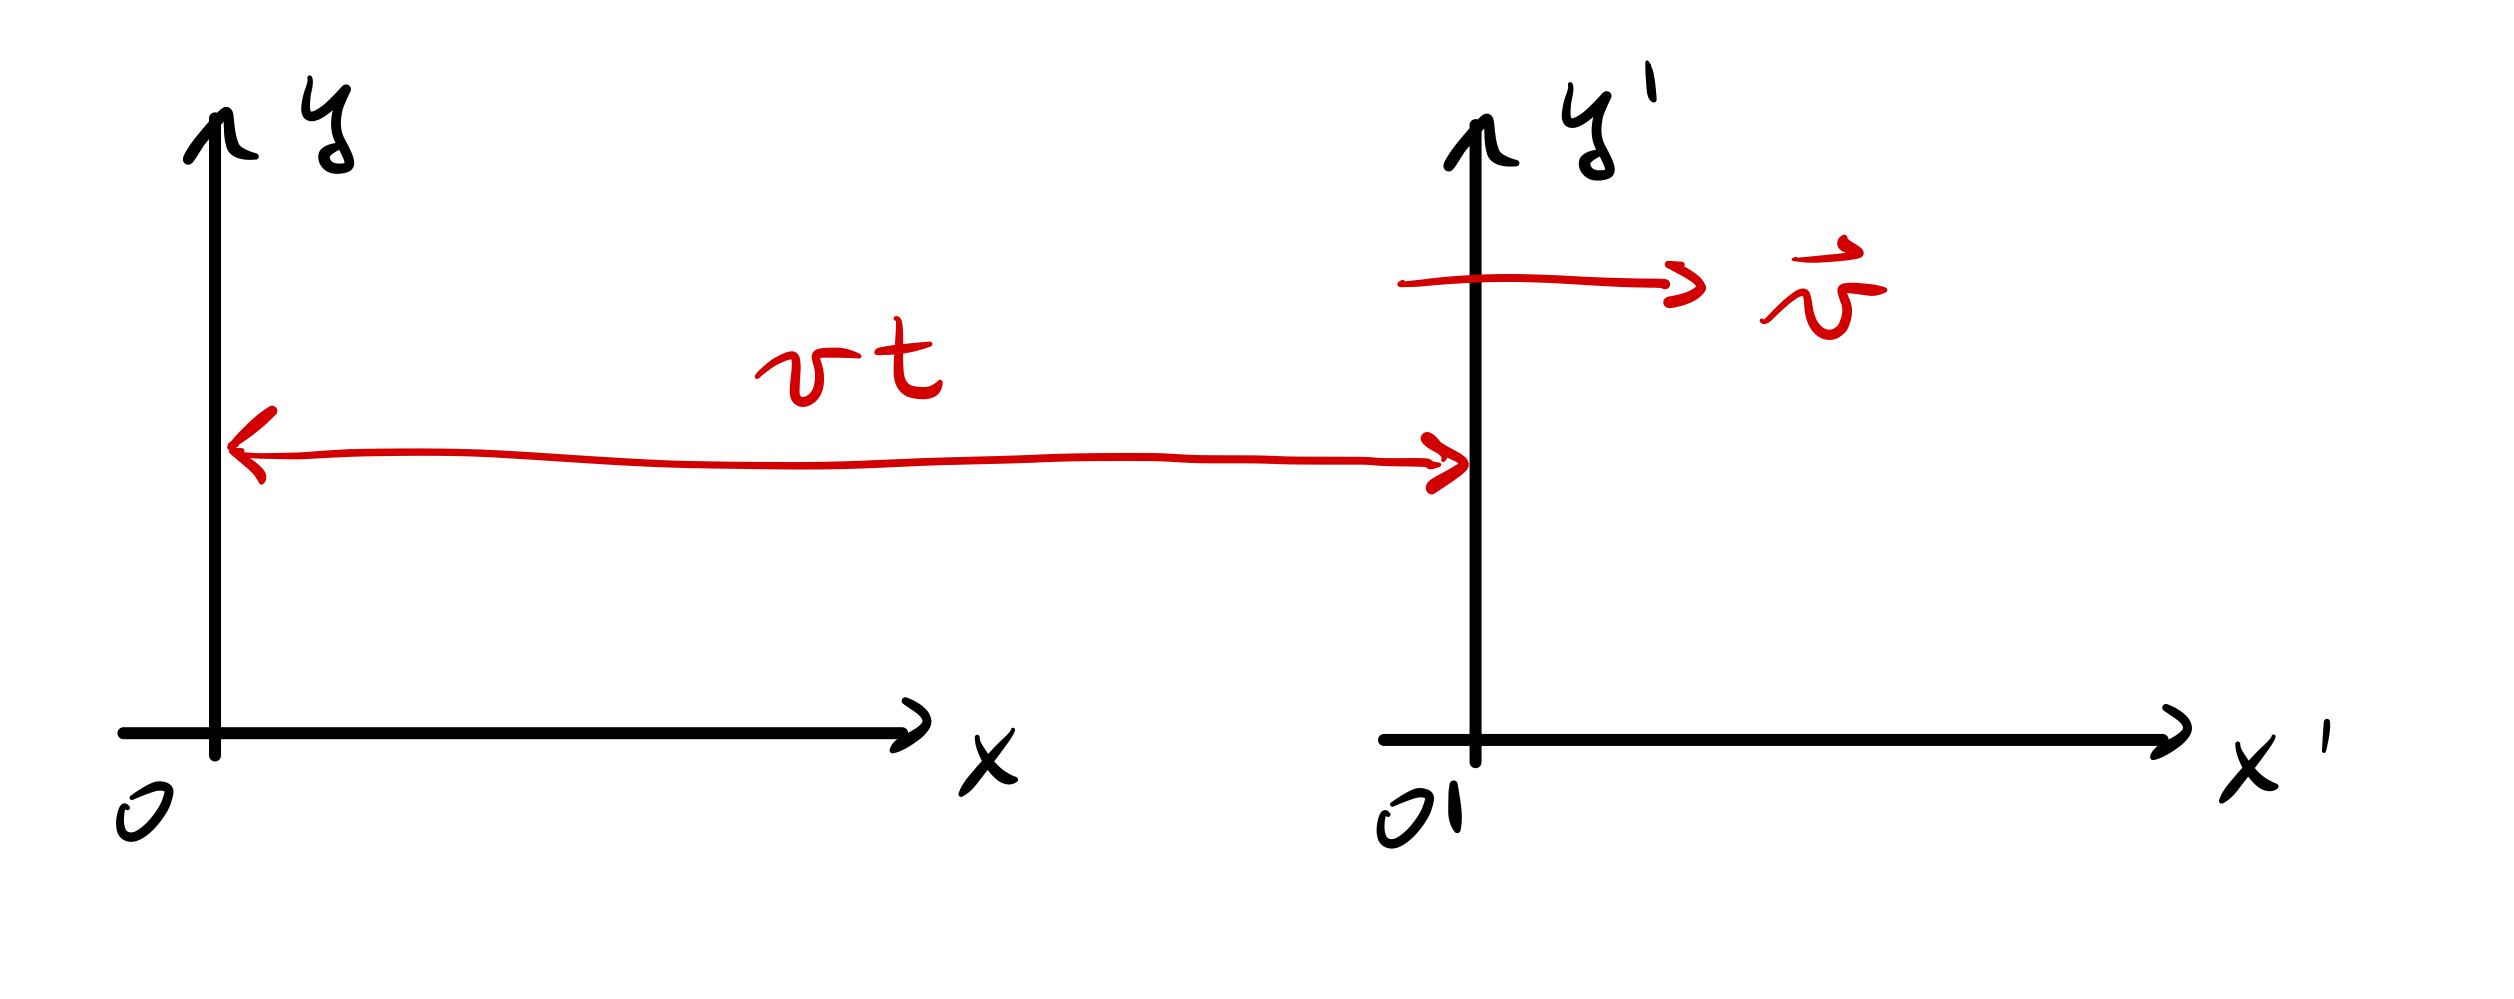
\includegraphics[scale=0.1]{img/Lorentz.jpeg}
    \caption{Dos sistemas de referencia conectados por un boost.}
    \label{fig:2.1}
\end{figure}

La transformación en este caso queda
\begin{align}
    ct'&=\gamma(ct-\beta x)\\
    x'&=\gamma(x-\beta ct)\\
    y'&=y\\
    z'&=z
\end{align}
donde el factor de Lorentz $\gamma$ está dado por
\begin{equation}
    \gamma =\frac{1}{\sqrt{1-\beta^2}}=\frac{1}{\sqrt{1-v^2/c^2}}
\end{equation}
Usando índices, esto queda
\begin{equation}\label{2.36}
\begin{split}
    x'^0&=\gamma(x^0-\beta x^1)\\
    x'^1&=\gamma(x^1-\beta x^0)\\
    x'^2&=x^2\\
    x'^3&=x^3
\end{split}
\end{equation}
Notemos que las coordenadas ortogonales a la dirección del boost permaneces invariantes. Las transformaciones de Lorentz inversas nos entregan los valores de las coordenadas $x$ en términos de las coordenadas $x'$. El resultado es el mismo conjunto de transformaciones con $x$ y $x'$ intercambiados y con $\beta$ reemplazado por $(-\beta)$.

Notemos que estas transformaciones satisfacen
\begin{equation}\label{2.37}
    (x^0)^2-(x^1)^2-(x^2)^2-(x^3)^2=(x'^0)^2-(x'^1)^2-(x'^2)^2-(x'^3)^2
\end{equation}
Por definición, \textcolor{purple}{\textit{las transformaciones de Lorentz son las transformaciones de coordenadas lineales e invertibles que respetan (\ref{2.37})}}.

En geenral, escribimos las transformaciones de Lorentz como la combinación lineal
\begin{equation}
    x'^\mu=\tensor{L}{^\mu_\nu}x^\nu
\end{equation}
donde las entradas $\tensor{L}{^\mu_\nu}$ son constantes que defines la transformación lineal. Para los boost en (\ref{2.36}), tenemos
\begin{equation}
    [L]=\tensor{L}{^\mu_\nu}=\mqty(\gamma&-\gamma\beta&0&0\\-\gamma\beta&\gamma&0&0\\0&0&1&0\\0&0&0&1)
\end{equation}
Además lo coeficientes $\tensor{L}{^\mu_\nu}$ están constreñidos por (\ref{2.37}) y deben satisfacer
\begin{equation}
    \tensor{L}{^\mu_\alpha}\eta_{\mu\nu}\tensor{L}{^\nu_\beta}=\eta_{\alpha\beta}
\end{equation}
En forma matricial, esta ecuación se puede escribir como
\begin{equation}
    L^T\eta L=\eta
\end{equation}
Una propiedad importante de las transformaciones de Lorentz puede ser deducida al tomar el determinante a ambos lados de la ecuación anterior, utilizando el hecho de que el determinante de un producto es el producto de los determinantes,
\begin{equation}
    \det L=\pm 1
\end{equation}

El conjunto de transformaciones de Lorentz incluye los boosts a lo largo de cada coordenadas espacial y las rotaciones de las coordenadas espaciales.

Cualquier conjunto de cuatro cantidades que transforma bajo transformaciones de Lorentz de la misma manera que los $x^\mu$ se dice que es un 4-vector, o un vector de Lorentz.

Un 4-vector $a^\mu$ se dice que es tipo-tiempo si $a^2=a\cdot a<0$, tipo-espacio si $a^2>0$, y nulo si $a^2=0$. 

\section{Coordenadas del cono de luz}
Ahora discutiremos un sistema de coordenadas extremadamente útil al momento de estudiar la teoría de cuerdas, el sistema de coordenadas del cono de luz. La cuantización de la cuerda relativista puede ser realizado directamente usando estas coordenadas.

Definimos las dos coordenadas del cono de luz $x^+$ y $x^-$ como dos combinaciones lineales independientes de la coordenadas temporal y una coordenada espacial, digamos $x^1$. Esto se escribe como
\begin{equation}\label{2.48}
\boxed{\begin{split}
    x^+&\equiv\frac{1}{\sqrt{2}}(x^0+x^1)\\
    x^-&\equiv\frac{1}{\sqrt{2}}(x^0-x^1)
\end{split}}
\end{equation}

\begin{figure}[h!]
    \centering
    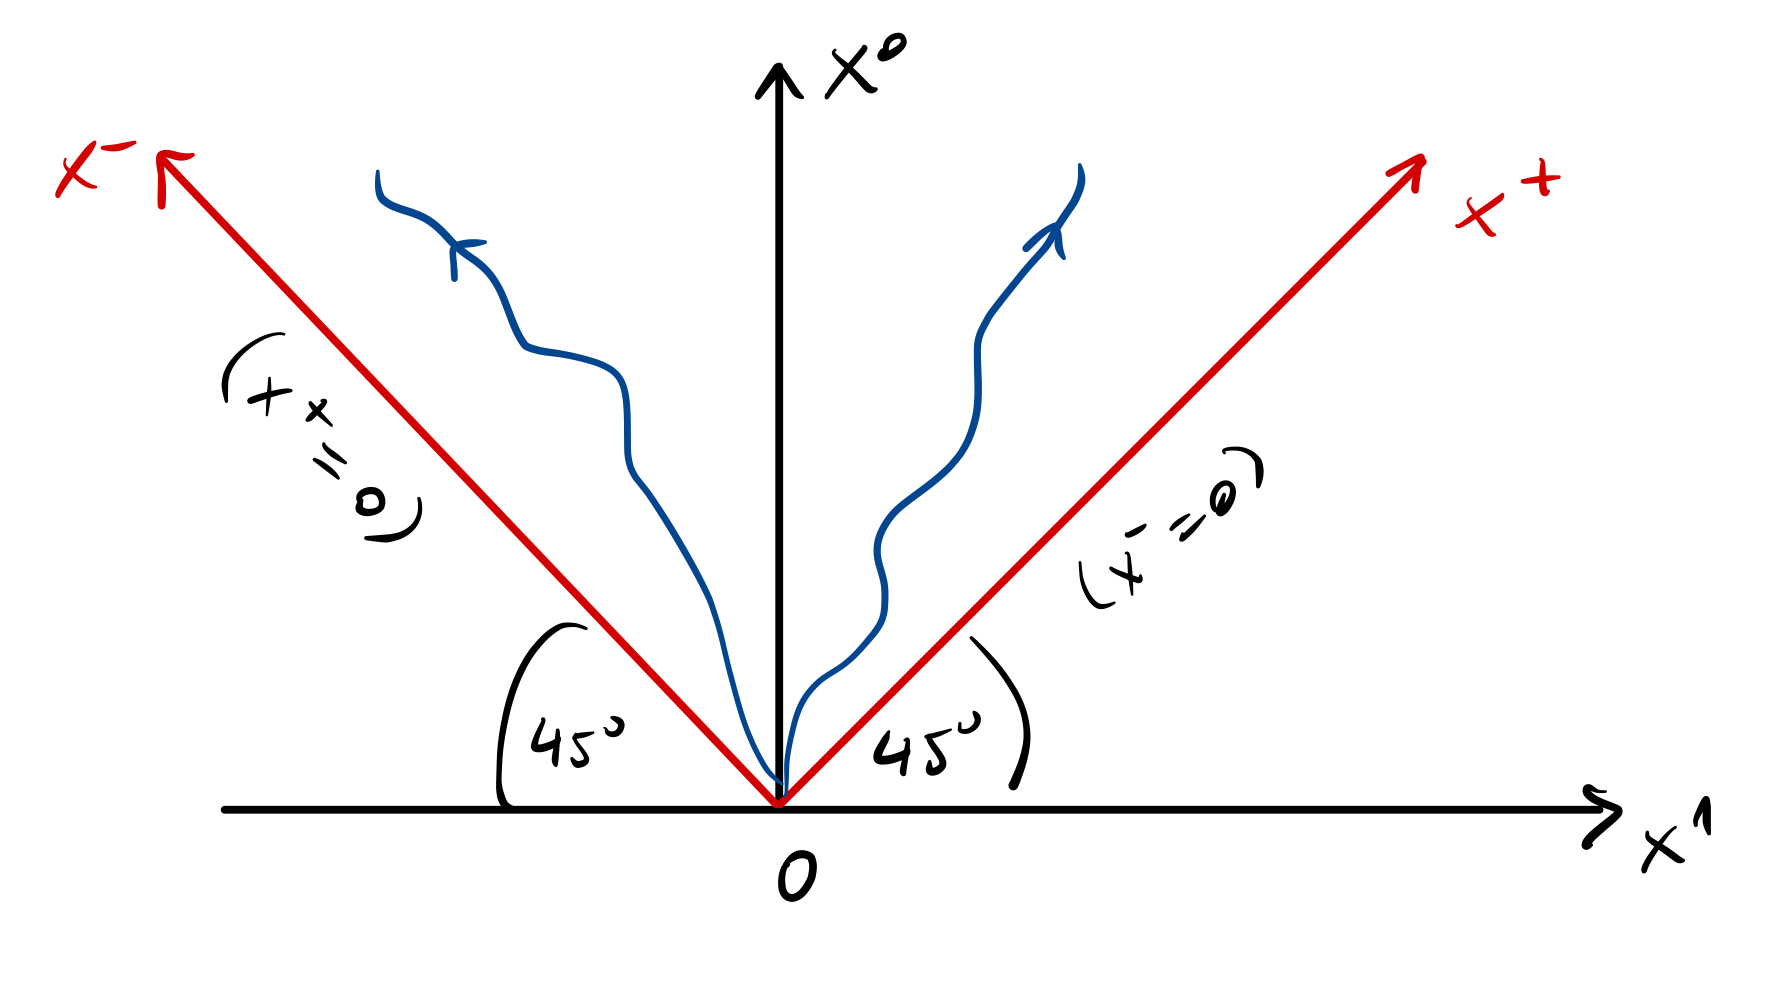
\includegraphics[scale=0.15]{img/light-cone coord.jpg}
    %\caption{Caption}
    %\label{fig:enter-label}
\end{figure}
En estas coordenadas, $(x^0,x^1)$ son tratadas como $(x^+,x^-)$, pero las otras dos coordenadas $x^2,x^3$ se mantienen. Así, el conjunto completo de coordenadas de cono de luz es $(x^+,x^-,x^2,x^3)$.

Las nuevas coordenadas $x^+$ y $x^-$ son llamadas coordenada de cono de luz porque los ejes coordenados asociados son las lineas de mundo de haces de luz emitidos desde el origen a lo largo del eje $x^1$. Para un hza de luz moviéndose en la dirección $x^1$ positiva, tenemos $x^1=ct=x^0$, luego $x^-=0$. La línea $x^-=0$ es, por definición, el eje $x^+$. Para un haz de lux moviéndose en la dirección $x^1$ negativa, tenemos $x^1=-ct=-x^0$, luego $x^+=0$. Esto corresponde al eje $x^-$, Los ejes $x^{\pm}$ son lineas a $45\degree$ con respecto a los ejes $x^0$ y $x^1$.

\begin{pregunta}
    ¿Podemos pensar a $x^+$, o quizás a $x^-$, como una nueva coordenada temporal?
\end{pregunta}
Yes. De hecho, ambas tienen el mismo derecho de ser llamadas coordenada temporal, a pesar de que ninguna lo es, en el sentido estándar de la palabra. Tiempo del cono de luz ya no es más el tiempo ordinario. Quizás la propiedad más familiar del tiempo es que este siempre avanza para cualquier movimiento físico de una partícula. Para todas esas curvas, tanto $x^+$ como $x^-$ incrementan a medida seguimos las flechas. La única sutileza es que, para rayos de luz especiales, el cono de luz se congelará. Como vimos, $x^+$ permanece constante para un rayo de luz en la dirección negativa de $x^1$, mientras que $x^-$ permanece constante para un rayo de luz en la dirección positiva de $x^+$.

Por definición, tomaremos $x^+$ como la \textit{coordenada temporal del cono de luz}. Luego, pensaremos a $x^-$ como la coordenada espacial. Por supuesto, estas coordenadas temporal y espacial del cono de luz serán algo extrañas. 

Tomando diferenciales de (\ref{2.48}),
\begin{equation}
    2dx^+dx^+=(dx^0+dx^1)(dx^0-dx^1)=(dx^0)^2-(dx^1)^2.
\end{equation}
Se sigue que el intervalo invariante, expresado en términos de estas coordenadas queda
\begin{equation}\label{2.50}
    \boxed{-ds^2=-2dx^+dx^-+(dx^2)^2+(dx^3)^2}
\end{equation}
La simetría en las definiciones de $x^+$ y $x^-$ es evidente. Notemos que, dado $ds^2$, resolviendo para $dx^-$ o para $dx^+$ no requiere que tomemos la raíz cuadrada. Esta es una característica muy importante de estas coordenadas como veremos más adelante.

\begin{pregunta}
    ¿Cómo podemos representar (\ref{2.50}) en notación de índices?
\end{pregunta}
Aún necesitaremos índices que corran por 4 valores, pero esta vez estos serán denotados por
\begin{equation}
    +,-,2,3
\end{equation}
Introducimos la métrica del cono de luz $\hat{\eta}$, la cual como la métrica de Minkowski, es definida simétrica bajo intercambio de sus índices. Expandiendo esta ecuación y comparando con (\ref{2.50}), encontramos
\begin{equation}
    \hat{\eta}_{+-}=\hat{\eta}_{-+}=-1,\qquad \hat{\eta}_{++}=\hat{\eta}_{--}=0
\end{equation}

En el subespacio de $(+,-)$, los elementos diagonales de la métrica del cono de luz se anulan, pero los de afuera de la diagonal no. Además encontramos que $\hat{\eta}$ no acopla el subespacio $(+,-)$ con el subespacio $(2,3)$:
\begin{equation}
    \hat{\eta}_{+I}=\hat{\eta}_{-I},\qquad I=2,3
\end{equation}
La representación matricial de la métrica del cono de luz es
\begin{equation}
    \hat{\eta}_{\mu\nu}=\mqty(0&-1&0&0\\-1&0&0&0\\0&0&1&0\\0&0&0&1)
\end{equation}

Las componentes del cono de luz de cualquier 4-vector son definidas análogamente a (\ref{2.48}):
\begin{equation}\label{2.56}
\begin{split}
    a^+\equiv\frac{1}{\sqrt{2}}(a^0+a^1)\\
    a^-\equiv\frac{1}{\sqrt{2}}(a^0-a^1)
\end{split}
\end{equation}
El producto escalar entre dos vectores, puede ser escrito usando las componentes del cono de luz,
\begin{equation}
    \boxed{a\cdot b=-a^-b^+-a^+b^-+a^2b^2+a^3b^2=\hat{\eta}_{\mu\nu}a^\mu b^\nu}
\end{equation}



\subsection{Energía y momentum relativista}
En relatividad especial hay una relación básica entre las masa en reposo $m$ de una partícula puntual relativista, su energía $E$, y su momentum relativista $\vb*{p}$, dada por
\begin{equation}
    \frac{E^2}{c^2}-\vb*{p}\cdot\vb*{p}=m^2c^2
\end{equation}
La energía y el momentum relativista están dados en términos de la masa en reposo y la velocidad por las siguientes relaciones familiares:
\begin{equation}
    E=\gamma mc^2,\qquad \vb*{p}=\gamma m\vb*{v}
\end{equation}
Así, podemos definir el 4-momentum como
\begin{equation}
    p^\mu=(p^0,p^1,p^2,p^3)\equiv\left(\frac{E}{c},p_x,p_y,p_z\right)
\end{equation}
Usando las últimas dos ecuaciones, tenemos
\begin{equation}
    p^\mu=\left(\frac{E}{c},\vb*{p}\right)=m\gamma(x,\vb*{v})
\end{equation}







\newpage
\printbibliography
\end{document}